\documentclass[a4paper,ngerman]{atseminar}

\usepackage{microtype}
\usepackage{graphicx}
\usepackage{algorithm2e}
\usepackage[left]{lineno}
\usepackage{tikz}
\usetikzlibrary{bayesnet}
\usepackage{wasysym}

\linenumbers

%% Please do not include packages that change the layout/size of the
%% of the document. They will be removed.

\bibliographystyle{plain}%the recommended bibstyle

% Preamble with header information 
\subject{Ausarbeitungen für das Seminar}
\title{Algorithmentechnik}
\titlerunning{Algorithmic Methods in the Humanities}%optional



\newcommand*{\vinput}[1]{\vcenter{\hbox{\input{#1}}}}
\newcommand*{\vpointer}{\vcenter{\hbox{\scalebox{1}{\Huge\pointer}}}}


%Organizer macros:%%%%%%%%%%%%%%%%%%%%%%%%%%%%%%%%%%%%%%%%%%%%%%%%%%%%%


%% do not use this field, but \summaryauthor
\author{}

%%%%%%%%%%%%%%%%%%%%%%%%%%%%%%%%%%%%%%%%%%%%%%%%%%%%%%%%%%%%%%%%%%%%%%%%%%%%%%%
%%%%%%%%%%%%%%%%%%%%%%%% begin of document %%%%%%%%%%%%%%%%%%%%%%%%%%%%%%%%%%%%
%%%%%%%%%%%%%%%%%%%%%%%%%%%%%%%%%%%%%%%%%%%%%%%%%%%%%%%%%%%%%%%%%%%%%%%%%%%%%%%
\begin{document}

\maketitle

%\GERMAN
\ENGLISH

%%%%% YOUR REPORT BEGINS HERE
\section{Latent Dirichlet Allocation}
\summaryauthor[Florian Becker]{Florian Becker}

\begin{abstract}
Latent Dirichlet Allocation .....
\end{abstract}

Hier steht der Inhalt der Ausarbeitung.

\subsection{Preliminaries and Notation}

\subsubsection{Multinomial Distribution}

The binomial distribution is a discrete distribution over binary events.	
\begin{align*}
\Pr(X = k) = \binom n k  p^k(1-p)^{n-k}
\end{align*}


\subsection{Dirichlet Distribution}
The Dirichlet distribution $Dir(\alpha)$ is a probability distribution parameterized by a positive real valued vector $\alpha$.
The probability density function is given by:

\begin{align*}
f \left(x_1,\cdots, x_{K}; \alpha_1,\cdots, \alpha_K \right) = \frac{\Gamma\left(\sum_{i=1}^K \alpha_i\right)}{\prod_{i=1}^K \Gamma(\alpha_i)} \prod_{i=1}^K x_i^{\alpha_i - 1}       \qquad\boldsymbol{\alpha}=(\alpha_1,\cdots,\alpha_K) 
\end{align*}


\subsubsection{Plate Notation}
In a probabilistic graphical model conditional dependence between various random variables are often depicted in plate notation.
Plate notation is a concise method for 

$\vinput{dependence_graph} \vpointer  \vinput{plate_dependence_graph}$


%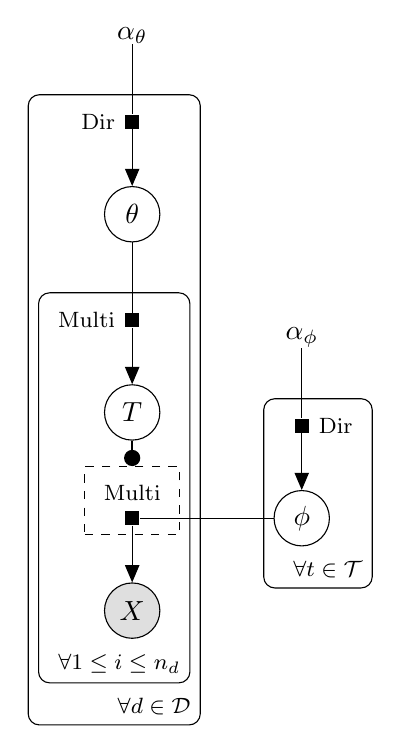
\begin{tikzpicture}[x=1.7cm,y=1.8cm]

  % Nodes

  \node[obs]                   (X)      {$X$} ; %
  \node[latent, above=of X]    (T)      {$T$} ; %
  \node[latent, above=of T]    (theta)  {$\theta$}; %
  \node[const, above=of theta] (atheta) {$\alpha_\theta$};


  % Factors
  \factor[above=of X]     {X-f}     {Multi} {} {} ; %
  \factor[above=of T]     {T-f}     {left:Multi} {} {} ; %
  \factor[above=of theta] {theta-f} {left:Dir} {} {} ; %

  % More nodes
  \node[latent, right=of X-f] (phi)  {$\phi$}; %
  \node[const, above=of phi]  (aphi) {$\alpha_\phi$}; %

  \factor[above=of phi] {phi-f} {right:Dir} {} {} ; %

  \factoredge {theta}  {T-f}     {T} ; %
  \factoredge {atheta} {theta-f} {theta} ; %
  \factoredge {phi}    {X-f}     {X} ; %
  \factoredge {aphi}   {phi-f}   {phi} ; %

  \gate {X-gate} {(X-f)(X-f-caption)} {T}

  \plate {plate1} { %
    (X)(X-gate) %
    (T)(T-f)(T-f-caption) %
  } {$\forall 1 \leq i \leq n_d$}; %
  \plate {} { %
    (plate1) %
    (theta)(theta-f)(theta-f-caption) %
  } {$\forall d \in \mathcal{D}$} ; %
  \plate {} { %
    (phi)(phi-f)(phi-f-caption) %
  } {$\forall t \in \mathcal{T}$} ; %

\end{tikzpicture}





\begin{figure}[h]
 \centering
 \includegraphics[scale = 0.7]{./picture}
 \caption{Dies ist die Beschreibung der Abbildung: Kurze Erklärung
was zu sehen ist.}
 \label{XY:fig:picture}
 % where X is the first letter of your first name and Y is the
% first letter of your last name.
\end{figure}

\begin{table}[h]
\centering
\caption{Tabellen haben Überschriften.}
\begin{tabular}{l|ll}
  \textbf{Zelle11} & \textbf{Zelle12} & \textbf{Zelle13} \\
  \hline
  \textbf{Zelle21} & Zelle22 & Zelle23 \\
  \textbf{Zelle31} & Zelle32 & Zelle33 \\
  
\end{tabular}
\label{XY:tab:interessant}
% where X is the first letter of your first name and Y is the
% first letter of your last name.
\end{table}



\begin{algorithm}[H]
\caption{Greedy}
\KwIn{Menge $\mathcal{C}$ aller Kreise in $G=(V,E)$.}
\KwOut{ Kreisbasis minimalen Gewichts von $G$.}
Sortiere $\mathcal{C}$ aufsteigend nach Gewicht zu $C_1,\ldots,C_k$\; 
$\mathcal{B}^\star$ $\leftarrow$ $\emptyset$\; %
  \For{$i = 1$ \KwTo $k$}{ %
    \If{$\mathcal{B}^\star \cup \{C_i\}$ linear unabhängig}{ %
      $B^\star$ $\leftarrow$ $B^\star \cup \{C_i\}$\; 
    }
} %
\end{algorithm}

\begin{theorem}[Titel des Theorems (optional)]
 Die Aussage des Theorems.
\end{theorem}

\begin{proof}
 Der Beweis für das Theorem.
\end{proof}

\begin{example}
 Dies ist ein Beispiel.
\end{example}


\begin{lemma}[Titel des Lemmas (optional)]
 Die Aussage des Lemmas
\end{lemma}

\begin{corollary}[Titel des Korollar (optional)]
 Ein Korollar.
\end{corollary}


\begin{definition}[Titel der Definition(optional)]
Inhalt der Definition
\end{definition}

Das erste Beispiel \cite{example1}, das zweite Beispiel
\cite{example2} und  das dritte Beispiel \cite{example3, example4}
für eine Referenz.

\subsection{Zweiter Abschnitt}


\begin{definition}[Titel der Definition(optional)]
Inhalt der Definition
\end{definition}





\bibliography{references}



%%%%% YOUR REPORT ENDS HERE




\end{document}
